\chapter{Link--Discovery--Durchführung}
\label{link_discovery}

Dieses Kapitel beschäftigt sich mit den konkret durchgeführten Schritten zur Link Discovery an Beispieldaten. Das Vorgehen und die verwendete Modellierung des Weltausschnittes wurde umfassend in \cref{ld_framework} beschrieben. Im Folgenden wird die initiale Erstellung des Weltausschnittes aus den Daten des Tagging--Systems von Spreadshirt, die Anreicherung durch Clicktracking--Daten, Zerlegung von Wortgruppen in Einzelwörter und Integration des Wortschatzes der Universität Leipzig beschrieben. Anschließend wird die konkrete Prioisierung der Beziehungen mittels evolutionärer Algorithen erläutert und die Ergebnisse der Link Discovery zusammenfassend ausgewertet.

\section{Initiale Erstellung des Weltausschnittes aus Tagging--Daten}
\label{ld_tags}

Die initiale Erstellung des Weltausschnittes stellt den ersten Schritt des in \cref{ld_process} definerten Link--Discovery--Prozesses dar. Die konkrete Datenquelle, die im Rahmen dieser Arbeit für diesen Schritt verwendet wurde, ist das Tagging--System des Unternehmens Spreadshirt, welches in \cref{tag_sprd} beschrieben wurde. Aus diesen Daten wird mittels Kookkurrenz (siehe \cref{co-occurence}) ein Graph erstellt, der der in \cref{world_graph} erläuterten Repräsentation des Weltausschnittes entspricht. Dieser stellt die Grundlage für alle folgenden Anreicherungsschritte dar. Um diesen initalen Graphen zu berechnen, sind die in \cref{integration_generic} aufgeführten Schritte des Imports, der Bereinigung, der Reduktion, der Transformation und der Integration nötig. Die Umsetzung dieser Schritte wird im folgenden Abschnitt beschrieben.

\subsection{Import}

Die Daten liegen im Quellsystem, einer MySQL--Datenbank, in relationaler Form vor. Somit existieren, dem Datenmodell von Tagging--Systemen in \cref{tagging_data} folgend, Tabellen für Benutzer, Tags, Dokumente und Taggings. Da der Inhalt der Dokumente sowie die Benutzer für die Kookkurrenzberechnung nicht relevant sind, genügt der Import der Tabellen \emph{Tags} und \emph{Taggings}. Das Datenmodell der für den Import benötigten Daten ist in \cref{fig:tag_source_erd} dargestellt.

\begin{figure}[h]
\centering
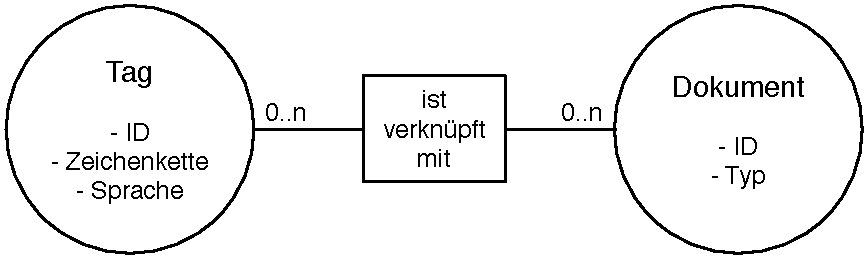
\includegraphics[width=0.6\textwidth]{tag_source_erd}
\caption{FMC--Entity--Relationship--Diagramm der Tagging--Quelldaten}
\label{fig:tag_source_erd}
\end{figure}

Die Tags besitzen, neben einem eindeutigen Bezeichner, die Attribute \emph{tag} für die Zeichenkette und \emph{lang} für die Sprache des Tags. \cref{lst:tag_import_tag} zeigt beispielhaft eine solche Tag--Entität.

\begin{lstlisting}[language=json, label={lst:tag_import_tag}, caption={JSON--Beispiel für einen importierten Tag}, float=h]
{
    "tag_id": 12345,
    "tag": "segeln",
    "lang": "de"
}
\end{lstlisting}

Ein Tagging ist über den eindeutigen Bezeichner des Tags und den eindeutigen Bezeichner des getaggten Dokumentes definiert. Der Schlüssel des Dokumentes setzt sich dabei aus den Attributen \emph{object\_type\_id} und \emph{object\_id} zusammen, da die Dokumente der Spreadshirt--Plattform verschiedene Typen wie  ``Artikel'' oder ``Design'' besitzen können. In \cref{lst:tag_import_link} ist ein Tagging beispielhaft dargestellt.

\begin{lstlisting}[language=json, label={lst:tag_import_link}, caption={JSON--Beispiel für ein importiertes Tagging}, float=ht]
{
    "object_id": 45678
    "object_type_id": 3,
    "tag_id": 12345
}
\end{lstlisting}

Gemäß des Mengengerüstes aus \cref{tag_amount} stehen nach dem Import \num{2072079} Tags und \num{71938905} Taggings für die folgenden Integrationsschritte zur Verfügung.

\subsection{Bereinigung}

An den Tagging--Daten liegen die in \cref{quality} genannten Defekte in Hinblick auf die Datenqualität vor. Diese sollten in einem Bereinigungsschritt reduziert werden. Hierbei liegt das Hauptaugenmerk auf der Erkennung von Duplikaten und später nicht verwertbaren Zeichenketten. Alle durchgeführten Maßnahmen zur Bereinigung beziehen sich hierbei auf das Attribut \emph{tag} eines Tag--Objektes, also der Zeichenkette selbst.

In den unbereinigten importierten Daten existieren keine Duplikate in der Art, dass eine Paarung aus Zeichenkette und Sprache immer nur genau einmal in den Daten vorhanden ist. Jedoch enthalten viele der Tags nicht weiter verwertbare Zeichen wie nicht druckbare ASCII Zeichen, Anführungszeichen, Satzzeichen, Sonderzeichen sowie überflüssige Leerzeichen am Anfang und Ende der Zeichenkette. Außerdem existiert in den importierten Daten eine Unterscheidung zwischen Groß- und Kleinschreibung. Diese Unterscheidung bringt im Kontext der Link Discovery keine Vorteile und kann somit entfernt werden.

\begin{table}[h]
\centering
% \arraystretch}{1.3}
\begin{tabular}{lcl}
    \toprule
    Rohdaten & \phantom{abc} & Bereinigte Daten \\
    \midrule
    \textbackslash u0003\textbackslash r\textbackslash nregenbogen && regenbogen \\
    RegenBogen && regenbogen \\
    "Regenbogen" && regenbogen \\
    regenbogen +einhorn && regenbogen einhorn\\
    \phantom{abc} regenbogen && regenbogen \\
    regenbogen && regenbogen \\
    \bottomrule
\end{tabular}
\caption{Beispiele für die Tag--Bereinigung}
\label{tab:tag_cleaning}
\end{table}

Somit besteht der Bereinigungsschritt darin, nicht verwertbare Zeichen zu entfernen und alle Großbuchstaben in Kleinbuchstaben umzuwandeln. Dadurch entstehen Duplikate, welche im darauf folgenden Reduktionsschritt zusammengeführt werden können. In \cref{tab:tag_cleaning} sind einige Beispiele für die Bereinigungen aufgeführt. Dabei ist gut zu erkennen, dass durch die Bereinigungen Duplikate erzeugt werden.

\subsection{Reduktion}

Der Reduktionsschritt dient zur Einschränkung der Gesamtdaten auf eine nützliche oder handhabbare Menge. Außerdem kann durch Reduktion auch die Datenqualität verbessert werden.

Im Fall der Tagging--Daten liegt das Hauptaugenmerk im Reduktionsschritt auf der Entfernung von Duplikaten, die bei der Bereinigung entstanden sind. Gleichzeitig muss sicher gestellt werden, dass keine Informationen über die Verwendung der Tags verloren gehen. Somit besteht die Duplikatentfernung der Tags im Zusammenführen von Datensätzen mit gleichen Zeichenketten und Sprachen. Gleichzeitig werden auch die Taggings zusammengeführt.

\begin{figure}[h]
\centering
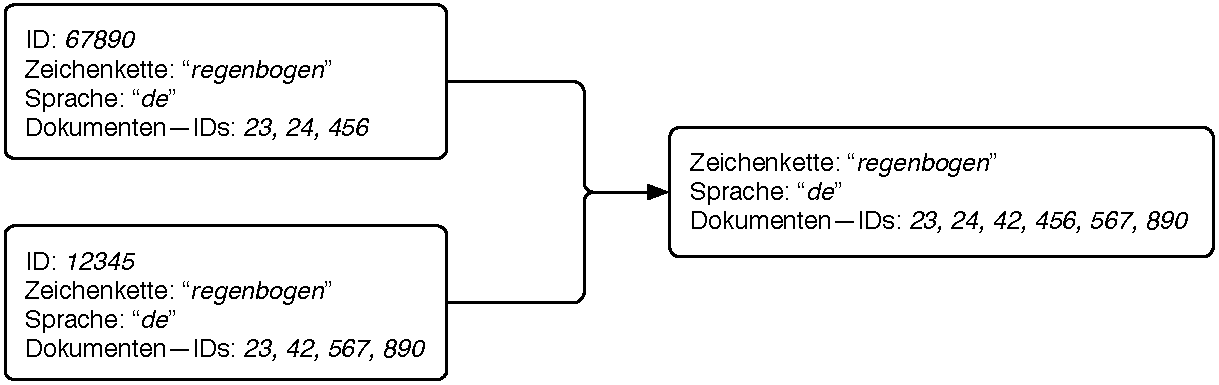
\includegraphics[width=0.9\textwidth]{tag_reduction}
\caption{Beispiel für das Zusammenführen der bereinigten Tags}
\label{fig:tag_reduction}
\end{figure}

Werden die Verknüpfungen zweier Tags mit Dokumenten zusammengeführt, können auch dabei wieder Duplikate entstehen. Diese müssen in diesem Fall entfernt werden, da ein Tag nicht mehrmals mit einem Dokument verknüpft werden kann. Das Zusammenführen von Tags ist exemplarisch in \cref{fig:tag_reduction} dargestellt.

Dabei findet ebenfalls eine Denormalisierung der Daten statt, da alle Dokumente, für die ein Tag vergeben werden, direkt mit in das Tag--Objekt gespeichert werden. Dies ist beispielhaft in \cref{lst:tag_denormalization} abgebildet. Das Attribut \emph{links} enthält alle Verknüpfungen des Tags mit Dokumenten.

\begin{lstlisting}[language=json, label={lst:tag_denormalization}, caption={JSON--Beispiel für die denormalisierten Tagging-Daten}, float=t]
{
    "string": "segeln"
    "language": "de",
    "links": [
        {
            "object_id": 45678, 
            "object_type_id": 3
        },
        {
            "object_id": 98764, 
            "object_type_id": 4
        },
        ...
    ]
}
\end{lstlisting}

Eine weitere im Rahmen dieser Arbeit unternommene Maßnahme zur Datenreduktion bestand darin, sich auf die Menge der Tags zu beschränken, deren Attribut \(lang\) den Wert \emph{de} besitzt. Praktisch handelt es sich um alle Tags, die als deutsch gekennzeichnet in der Datenbank gespeichert sind. Diese Einschränkung wurde vorgenommen, um die zu verarbeitende Datenmenge überschaubar zu halten. Außerdem wird dadurch der nationale Kontext, in dem die Begriffe verwendet wurden, weitestgehend beibehalten.

Ein letzter Reduktionsschritt besteht in der Entfernung der Tags, deren Zeichenketten eine Länge von \num{1} besitzen, da in der deutschen Sprache keine einbuchstabigen Wörter existieren.

Nach der beschriebenen Reduktion befinden sich noch \num{314351} Tags und \num{23255714} Taggings in der Datenbank. Dies entspricht einer Reduktion von ca. \num{68} Prozent gegenüber der importierten Menge von Objekten.

\subsection{Transformation}

Der Transformationsschritt stellt die Überführung der Daten in die in \cref{world_graph} beschriebene Repräsentation des Weltausschnittes dar. Für die Tagging--Daten bedeutet dies eine Umformung in eine Graphenform, wobei die Kanten des Graphen über Kookkurrenz ermittelt werden. Die genaue Umsetzung dieser Transformation mittels des MapReduce--Programmiermodells wird in \cref{mapreduce_cooccurence} detailliert beschrieben.

Je Tag wird ein während der Transformation ein Knotenobjekt erzeugt. Dieses besitzt als benötigte Attribute die \emph{Zeichenkette} und die \emph{Sprache} des Tags, aus dem es erzeugt wurde und repräsentiert somit einen Begriff des Weltausschnittes. Außerdem wird ein Kontext dieses Begriffes im Rahmen des Tagging--Systems erzeugt. Dieser enthält die Anzahl der Verwendungen des Begriffes als Tag und die eindeutigen Bezeichner der Dokumente, also der Artikel und Designs, die mit dem Begriff getaggt wurden. Weiterhin wird für jedes Knotenobjekt ein global eindeutiger Bezeichner generiert, um die spätere Referenzierungs der Knoten zu ermöglichen. \cref{lst:tag_transform_node} zeigt ein Beispiel für ein so erzeugtes Knotenobjekt.

\begin{lstlisting}[language=json, label={lst:tag_transform_node}, caption={JSON--Beispiel für einen aus den Tagging--Daten erzeugten Knoten}, float=h]
{
    "_id" : ObjectId("51efc20147cae77dfc02e0ac"),
    "language" : "de",
    "string" : "mama",
    "tagProperties" : {
        "occurenceCount" : 3,
        "articleCount" : 2,
        "designCount" : 1,
        "articleIDs" : [
            24231101,
            24231105
        ],
        "designIDs" : [
            15514592
        ]
    }
}
\end{lstlisting}

Die Erzeugung der Kanten erfolgt wie in \cref{mapreduce_cooccurence} beschrieben. Für jedes gemeinsame Auftreten von zwei Tags werden zwei Kantenobjekte erzeugt. Diese beschreiben gerichtete Kanten zwischen den Begriffen, die ein gemeinsames Auftreten der Tags repräsentieren. Neben den eindeutigen Bezeichnern der Quell- und Zielknoten enthält das Kantenobjekt den Kantentyp \emph{Tagging--Kookkurrenz} sowie die absolute Anzahl gemeinsamer Vorkommen der Tags und die in \cref{measures} beschriebenen Kookkurrenzmaße. Außerdem erhält die Kante selbst einen global eindeutigen Bezeichner zur Referenzierung. Ein Beispiel für eine aus den Tagging--Daten erzeugte Kante ist in \cref{lst:tag_transform_edge} dargestellt.

\begin{lstlisting}[language=json, label={lst:tag_transform_edge}, caption={JSON--Beispiel für eine aus den Tagging--Daten erzeugte Kante}, float]
{
    "_id" : ObjectId("51efd6f61177ff360605bd99"),
    "source" : ObjectId("51efc1af47cae77dfc00c3f8"),
    "target" : ObjectId("51efc1e047cae77dfc02087c"),
    "type" : "tag-co-occurence",
    "occurences" : 1,
    "dice" : 0.0001317089232795522,
    "jaccard" : 0.00006585879873551106,
    "cosine" : 0.008115343414514944
}
\end{lstlisting}

\subsection{Integration}

Da es sich bei der Integration der Tagging--Daten um die initiale Erstellung des Weltausschnittes handelt, ist der letzte Schritt trivial. Die transformierten Daten müssen lediglich in die Zieldatenbank kopiert werden, da noch keine weiteren Daten vorhanden sind, mit denen sie integriert werden müssen.

\subsection{Ergebnisse}
\label{tagging_results}

Durch die Schritte, die zur Link Discovery aus den Tagging--Daten verwendet wurden, wurden insgesamt \num{314351} Knoten und \num{21834868} Kanten erzeugt.

Eine mögliche Metrik für die quantitativen Eigenschaften der Ergebnisse ist die Verteilung der ausgehenden Kanten, die jeder Knoten besitzt. Diese ist als Histogramm in \cref{fig:hist_only_tags} dargestellt. Hierbei ist anzumerken, dass die Klassen des Histogrammes exponentiell breiter werden, um Knoten, die sehr viele Kanten besitzen, im Histogramm darstellen zu können.

\begin{figure}[ht]
\centering
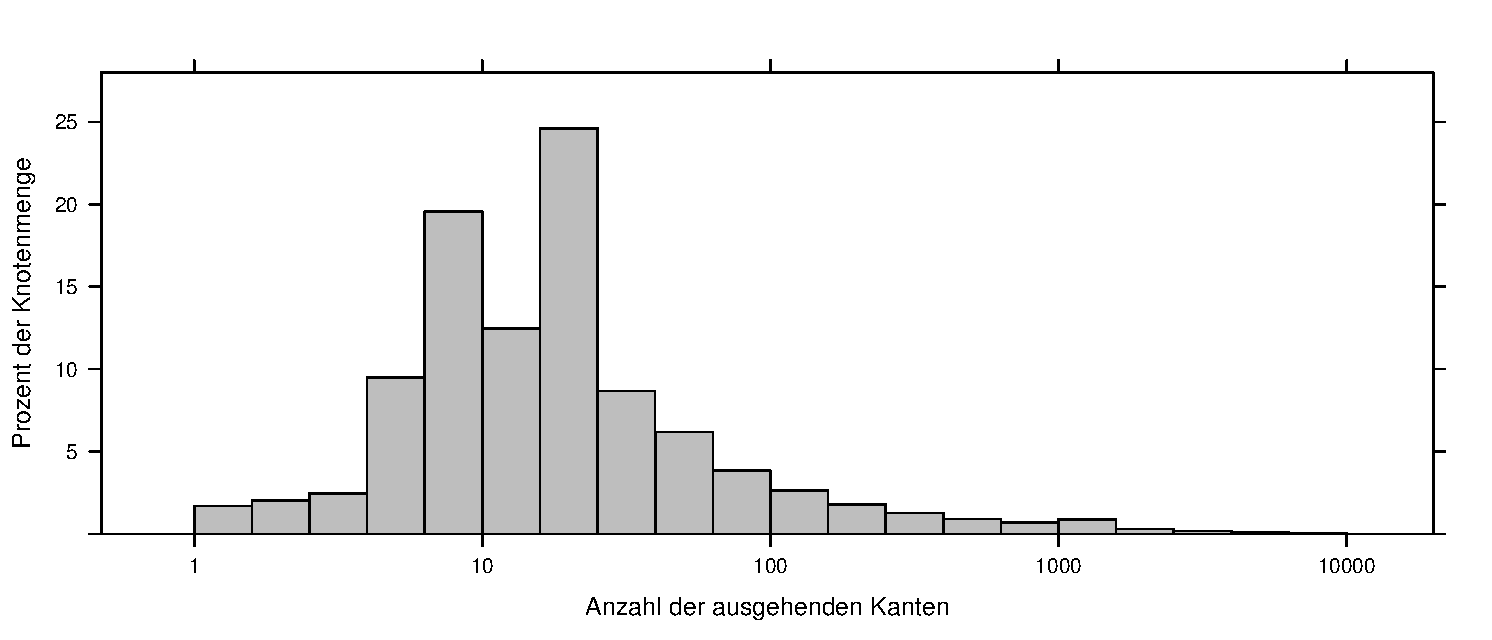
\includegraphics[width=\textwidth]{hist_only_tags}
\caption{Histogramm der Verteilung der Tagging--Kookkurrenz--Kanten}
\label{fig:hist_only_tags}
\end{figure}

\cref{tab:only_tags} zeigt die statistischen Kennzahlen Minimum, erstes Quartil, Median, drittes Quartil, Maximum und Durchschnitt der Verteilung der Kanten nach Berechnung der Tagging--Kookkurrenz.

\begin{table}[ht]
\centering
\begin{tabular}{lr}
    \toprule
    Kennzahl & Wert \\
    \midrule
    \(min\) & \num{0} \\
    \(Q_{0.25}\) & \num{9} \\
    \(Q_{0.5}\) & \num{16} \\
    \(Q_{0.75}\) & \num{29} \\
    \(max\) &  \num{35169} \\
    \(avg\) &  \num{74,64} \\
    \bottomrule
\end{tabular}
\caption{Statistische Kennzahlen für die Verteilung der Tagging--Kookkurrenz--Kanten}
\label{tab:only_tags}
\end{table}

Bei der Interpretation dieser Daten fällt auf, dass die Anzahl der ausgehenden Kanten sehr ungleich verteilt ist. Es existieren sehr viele Knoten mit wenigen Kanten und sehr wenige Knoten mit vielen Kanten. Der verhältnismäßig hohe Median sagt allerdings ebenfalls aus, dass die Hälfte aller Knoten mehr als \num{16} ausgehende Kanten besitzen. Dies lässt jedoch keine Aussage über die inhaltliche Qualität der erzeugten Zusammenhänge zu. Diese kann nur auf Basis eines einzelnen Begriffes und dessen Beziehungen beurteilt werden.

Der Begriff, der das Maximum von \num{35169} ausgehenden Kanten erreicht, ist der Begriff ``liebe''. Dieser Begriff zählt zu den meistgesuchten und verwendeten Tags auf der Spreadshirt--Plattform. Dies spiegelt sich offensichtlich auch darin wieder, dass er zusammen mit \num{35169} anderen unterschiedlichen Tags vergeben wurde.

Nachdem in diesem Abschnitt die Integration der Tagging--Daten beschrieben wurde, beschäftigt sich der folgende Abschnitt mit der Anreichung des Weltausschnittes mit den Daten des Clicktracking--Systems von Spreadshirt.

\section{Anreicherung des Weltausschnittes mit Clicktracking--Daten}
\label{clicktracking}

Spreadshirt betreibt ein Clicktracking--System (siehe \cref{clicktracking_theo}), welches die Klicks der Benutzer auf Artikel und Designs auf Suchergebnisseiten aufzeichnet. Dabei ist unerheblich, ob der Benutzer bei Spreadshirt registriert und angemeldet ist. Dieses System sammelt Daten von beiden Spreadshirt--Plattformen (siehe \cref{platforms}). In \cref{fig:search_result} ist beispielhaft eine Suchergebnisseite der Spreadshirt--Plattform abgebildet, welche die gefundenen Designs für eine Suchanfrage auflistet.

\begin{figure}[t]
\centering
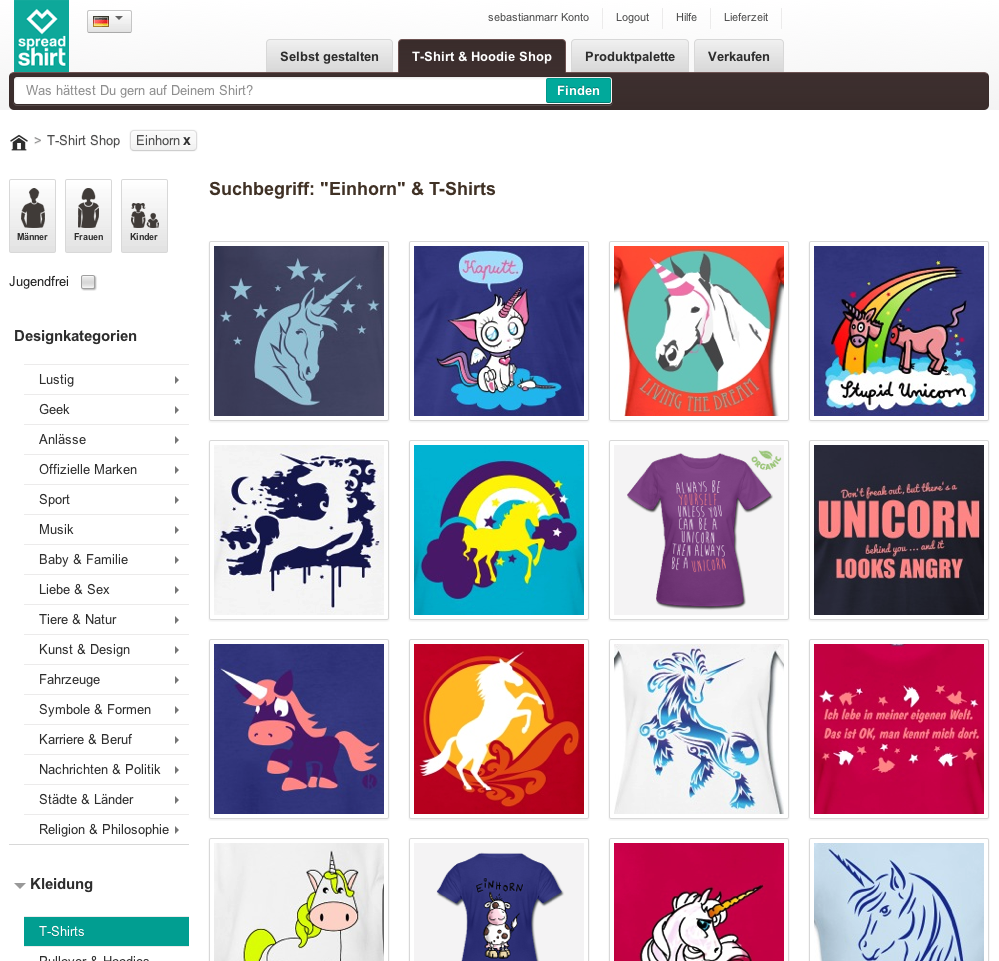
\includegraphics[scale=0.25]{search_result}
\caption{Beispiel für eine Spreadshirt--Suchergebnisseite}
\label{fig:search_result}
\end{figure}

Die von diesem System erzeugten Daten können für die Link Discovery von großer Bedeutung sein, da sie eine andere Perspektive auf die Begriffe im Graphen liefern. Die Tags liefern die Sicht der Partner, also der Personen, die Inhalte hochladen und verkaufen möchten. Die Klicks beschreiben die Sicht der Käufer, also der Personen, die nach Inhalten suchen. Durch die Auswertung der Clicktracking--Daten ergibt sich also die Möglichkeit, eine Form der Validierung der durch Partner vergebenen Metadaten zu erhalten. Die Annahme hierbei ist, dass Käufer nur auf Suchergebnisse klicken, die eine inhaltliche Relevanz zum eingegebenen Suchbegriff besitzen und somit ihren Erwartungen bezüglich des Suchbegriffes gerecht werden.

Wie bereits für die Tagging--Daten, werden im Folgenden auch für das Clicktracking die Schritte Import, Bereinigung, Reduktion, Transformation und Integration (siehe \cref{integration_generic}) näher erläutert. Der Ansatz zur Erzeugung der Verbindungen ist, wie schon bei den Tagging--Daten, kookkurrenzbasiert.

\subsection{Import}
\label{click_import}

Das Clicktracking--System erzeugt Dateien im JSON--Format, die zu jedem Klick auf einer Ergebnisseite die wesentlichen Informationen enthalten. Pro Klick ist ein JSON--Dokument in den Dateien abgespeichert. Ein Beispiel für ein solches Dokument ist in \cref{lst:click_raw} dargestellt.

\begin{lstlisting}[language=json, label={lst:click_raw}, caption={JSON--Beispiel für ein Clicktracking--Rohdokument}, float]
{
    "date": "01.07.2013 00:09:31_633",
    "path": "/track/eu/205909/1E3B6E3E-4496-C51A14A8FA25/2.10.4/list",
    "params": {
        "locale": "[de_DE]",
        "search-query": "[biene]",
        "cl": "[a18869874, p25446183, i49]"
    }
}
\end{lstlisting}

Ein Clicktracking--Dokument enthält die Attribute \emph{Datum}, \emph{Pfad}, \emph{Gebietsschema}, \emph{Suchbegriff} und die Daten des eigentlichen Klicks, also den geklickten \emph{Artikel}, das geklickte \emph{Produkt} und den \emph{Index}, also die Position des geklickten Inhaltes auf der Suchergebnisseite. Die Unterscheidung zwischen Produkt und Artikel ist im Domänenmodell von Spreadshirt begründet (siehe auch \cref{spreadshirt}) und für die Link Discovery nicht von Interesse. Es genügt, den geklickten Artikel im Weiteren näher zu betrachten.

Auffällig ist, dass die Möglichkeiten des JSON--Formates bei der Speicherung der Klickdaten nicht vollständig ausgenutzt wurden. So sind die Werte, die das geklickte Dokument beschreiben, als Zeichenkette abgelegt und zusätzlich die eindeutigen Bezeichner mit einem Buchstaben versehen, der ihren Typ angibt. Des weiteren enthalten  das Gebietsschema und der Suchbegriff zusätzliche eckige Klammern. Diese Defekte sollten im Bereinigungsschritt beseitigt werden, um ein nutzbareres Datenformat zu erhalten.

Da das Clicktracking--System zum Zeitpunkt des Imports erst 3 Monate Daten aufzeichnete, standen \num{2249942} solcher Klickdokumente zur Verfügung.

\subsection{Bereinigung}

Im Bereinigungsschritt sollten zunächst die im vorherigen Abschnitt genannten Defekte an den Daten des Clicktracking--Systems beseitigt werden. Dazu gehört die Entfernung der eckigen Klammern in Suchbegriff und Gebietsschema und die Extraktion des eindeutigen Bezeichners des geklickten Artikels. Aus dem Gebietsschema ist nur die Sprache von Interesse. Außerdem wurden für den Suchbegriff die gleichen Bereinigungsoperationen wie für die Tagging--Daten vorgenommen, also die Entfernung von überflüssigen Leerzeichen, Groß-/Kleinschreibung, nicht druckbarer Sonderzeichen und Satzzeichen.

Im Bereinigungsschritt werden so auch einfacher verarbeitbare Dokumente erzeugt, da die Möglichkeiten des JSON--Formates besser ausgenutzt werden. \cref{lst:tag_cleanup} zeigt das Ergebnis der Bereinigung des in \cref{click_import} gezeigten Beispieldokumentes.

\begin{lstlisting}[language=json, label={lst:tag_cleanup}, caption={JSON--Beispiel für die Bereinigung der Clicktracking--Dokumente}, float]
{
    "_id": ObjectId("51e7b1e0417498f9c6868939"),
    "query" : "biene",
    "date" : "2013-07-01T00:09:31.633Z",
    "articleId" : 18869874,
    "index" : 57,
    "language" : "de"
}
\end{lstlisting}

\subsection{Reduktion}

Die Reduktion der Clicktracking--Daten besteht zum einen aus einer Duplikatentfernung, zum anderen aus der Einschränkung der Sprache.

Im Sinne der Kookkurrenz ist es nicht von Bedeutung, wenn Paare aus Suchbegriffen und geklickten Artikeln mehrfach auftauchen, da hierfür nur das gemeinsame Auftreten unterschiedlicher Suchbegriffe betrachtet wird. Somit besteht die Duplikatentfernung lediglich darin, aus mehrfach vorkommenden Artikel-/Klickpaaren genau eines auszuwählen.

Außerdem erfolgte, wie schon bei den Tag--Daten, eine Einschränkung auf Klicks, die als \emph{deutsch} gekennzeichnet sind.

Nach dem Reduktionsschritt verblieben zur Transformation noch \num{411341} Klicks.

\subsection{Transformation}

Der Transformationsschritt dient zur Umformung der Clicktracking--Daten in die Graphenrepräsentation des Weltausschnittes aus \cref{world_graph}. Diese Umformung wird durch die Ermittlung von Kookkurrenz durchgeführt. Diese bestimmt sich hierbei daraus, welche Suchbegriffe zum Klick auf einen Artikel geführt haben. Wird ein Artikel zu mehreren Suchbegriffen geklickt, liegt die Vermutung nah, dass zwischen den Suchbegriffen ein irgendwie gearteter Zusammenhang besteht.

Ziel der Transformation ist somit die Erzeugung von Knoten und Kanten. Die Knoten werden zusätzlich mit einem Kontext verknüpft, der die Eigenschaften des durch den Knoten repräsentierten Begriffes im Kontext des Clicktracking--Systems. Konkret sind dies die Artikel, die zu dem Begriff als Suchbegriff geklickt wurden. \cref{lst:click_node} zeigt einen aus den Clicktracking--Daten erzeugten Knoten.

\begin{lstlisting}[language=json, label={lst:click_node}, caption={JSON--Beispiel für ein aus den Clicktracking--Daten erzeugtes Knotenobjekt}, float]
{
    "_id": ObjectId("51e7f1e04146498f9c6868945"),
    "string": "biene",
    "language": "de",
    "clickProperties": [
        { "articleId": 4512 },
        { "articleId": 4794 },
        ...
    ]
}
\end{lstlisting}

Die Kanten besitzen die gleiche Form wie die Kookkurrenzkanten, die bei der Integration der Tagging--Daten erzeugt wurden. Lediglich der Typ der Kanten ist unterschiedlich und lautet \emph{Clicktracking--Kookkurrenz}. Ein Beispiel für eine solche Kante ist in \cref{lst:click_edge} dargestellt.

\begin{lstlisting}[language=json, label={lst:click_edge}, caption={JSON--Beispiel für ein aus den Clicktracking--Daten erzeugtes Kantenobjekt}]
{
    "_id": ObjectId("51e91aff3b6a20bfd68c468a")
    "source" : ObjectId("51e91af93b6a20bfd68b0bed"),
    "target" : ObjectId("51e91aff3b6a20bfd68c463e"),
    "type": "click-co-occurence",
    "occs" : 1,
    "dice" : 0.003883495145631068,
    "jaccard" : 0.0019455252918287938,
    "cosine" : 0.04410810913912309
}
\end{lstlisting}

Die Durchführung des Transformationsschrittes erfolgte mittels MapReduce (siehe \cref{mapreduce_cooccurence}). Dadurch wurden \num{92727} Knoten und \num{310860} Kanten erzeugt.

\subsection{Integration}
\label{click_integration}

Die Integration der erzeugten Daten stellt eine Vereinigung des vorhandenen Weltausschnittes mit dem im Transformationsschritt erzeugten Graphen dar.

Die Knotenmenge wird derart vereinigt, dasssie die Eigenschaft behält, dass Paare aus Sprache und Zeichenkette eindeutig sind. Somit werden bei bereits vorhandenen Knoten die zusätzlichen Informationen bezüglich des Clicktrackings als Attribute hinzugefügt. Existiert eine Kombination aus Sprache und Zeichenkette noch nicht im Zielgraph, so wird der entsprechende Knoten eingefügt.

Da die erzeugten Kanten einen noch nicht im Graph vorhandenen Typ besitzen, müssen keine Kanten zusammengeführt werden. Jedoch werden die Bezeichner der Ziel- und Quellknoten entsprechend angepasst, wenn bei der Integration der Knoten eine Zusammenführung stattgefunden hat.

\subsection{Ergebnisse}

Durch die auf die Clicktracking--Daten angewendeten Link--Discovery--Schritte wurden dem Weltausschnitt \num{78237} neue Begriffe und \num{310860} neue Zusammenhänge vom Type \emph{Clicktracking--Kookkurrenz} hinzugefügt.

Wie schon für die Tagging--Daten in \cref{tagging_results}, wird im folgenden die Verteilung der Clicktracking--Kanten je Knoten als Metrik für die Ergebnisse der Clicktracking--Integration verwendet. Diese ist in \cref{fig:hist_only_clicktracking} als Histogramm mit exponentiell wachsenden Klassen dargestellt.

\begin{figure}[t]
\centering
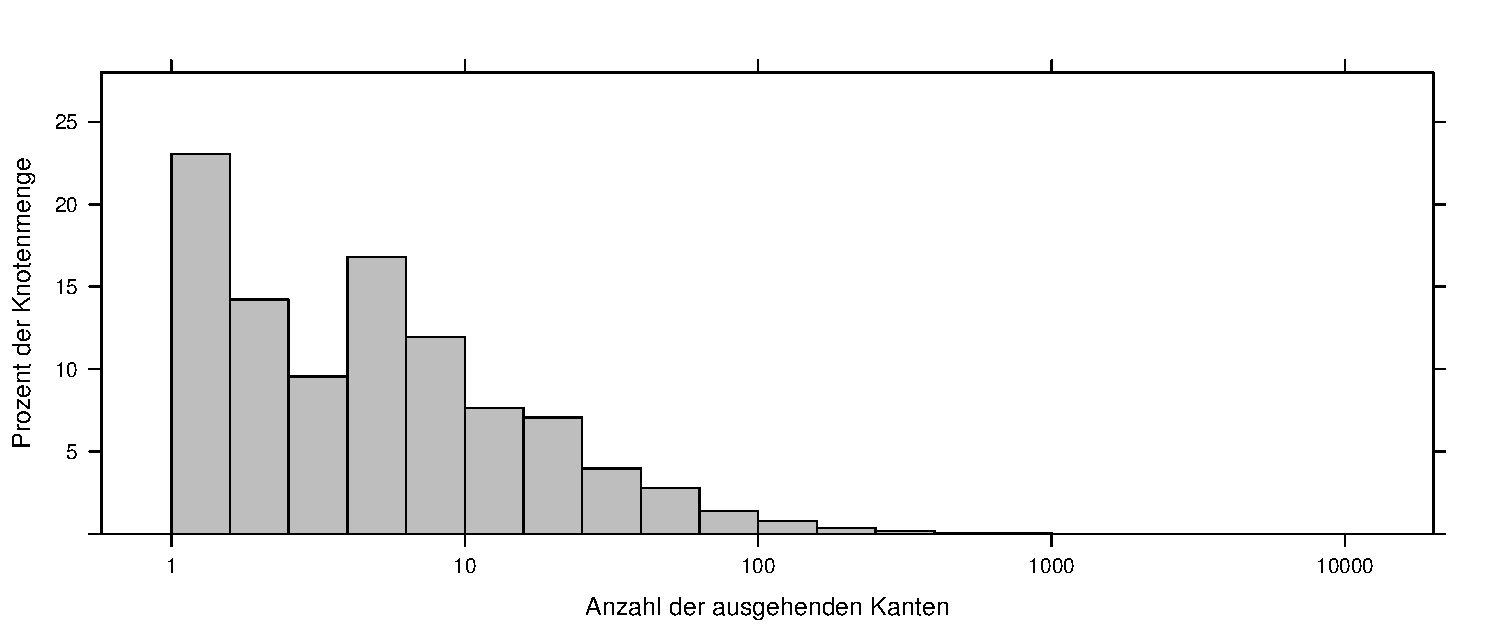
\includegraphics[width=\textwidth]{hist_only_clicktracking}
\caption{Histogramm der Verteilung der Clicktracking--Kookkurrenz--Kanten}
\label{fig:hist_only_clicktracking}
\end{figure}

\cref{tab:only_clicktracking} zeigt die statistischen Kennzahlen Minimum, erstes Quartil, Median, drittes Quartil, Maximum und Durchschnitt der Verteilung der Kanten nach Berechnung der Clicktracking--Kookkurrenz.

Bei der Interpretation dieser Daten fällt auf, dass im Vergleich zu den Tagging--Daten zum einen deutlich weniger Kanten, zum anderen auch durchschnittlich weniger Kanten pro Knoten erzeugt wurden. So muss bei circa einem Viertel der Knoten, die Kanten vom Typ Clicktracking--Kookkurrenz besitzen, mit zwei oder weniger Beziehungen gerechnet werden. Durch die geringe Kantenanzahl wird die Gesamtverteilung der Kanten jedoch nicht wesentlich beeinflusst (siehe \cref{lda_results}).

\begin{table}[h]
\centering
\begin{tabular}{lr}
    \toprule
    Kennzahl & Wert \\
    \midrule
    \(min\) & \num{1} \\
    \(Q_{0.25}\) & \num{2} \\
    \(Q_{0.5}\) & \num{4} \\
    \(Q_{0.75}\) & \num{10} \\
    \(max\) &  \num{1688} \\
    \(avg\) &  \num{12} \\
    \bottomrule
\end{tabular}
\caption{Statistische Kennzahlen für die Verteilung der Clicktracking--Kookkurrenz--Kanten}
\label{tab:only_clicktracking}
\end{table}

Nachdem die Anreicherung der Clicktracking--Daten durchgeführt wurde, beschäftigt sich der folgende Abschnitt mit der Anrreichung durch die Zerlegung von Wortgruppen in Einzelwörter.

\section{Anreicherung des Weltausschnittes durch Zerlegung von Wortgruppen}
\label{decomposition}

Die Zerlegung von Tags, die aus mehr als einem Wort bestehen, ist ein Anreicherungsschritt durch das Mining von schon im Weltausschnitt vorhandenen Daten (siehe \cref{enrichment_mining}). Neben der Erzeugung zusätzlicher Verbindungen ist er für weitere Integrationsschritte von Nutzen, da es Vorteile bringt, wenn möglichst viele Einzelwörter im Weltausschnitt gespeichert sind (siehe \cref{wortschatz}).

\subsection{Vorgehensweise}

Zum Zeitpunkt des Importes befanden sich \num{147364} Begriffe im Weltausschnitt, die aus mehreren Wörtern bestehen. Dies entspricht \num{47} Prozent aller bereinigten deutschen Tags. Dieser Umstand legt die Vermutung nahe, dass in diesen zusammengesetzten Tags auch Wörter enthalten sind, die nicht als Einzelwörter existieren.

\begin{figure}[h]
\centering
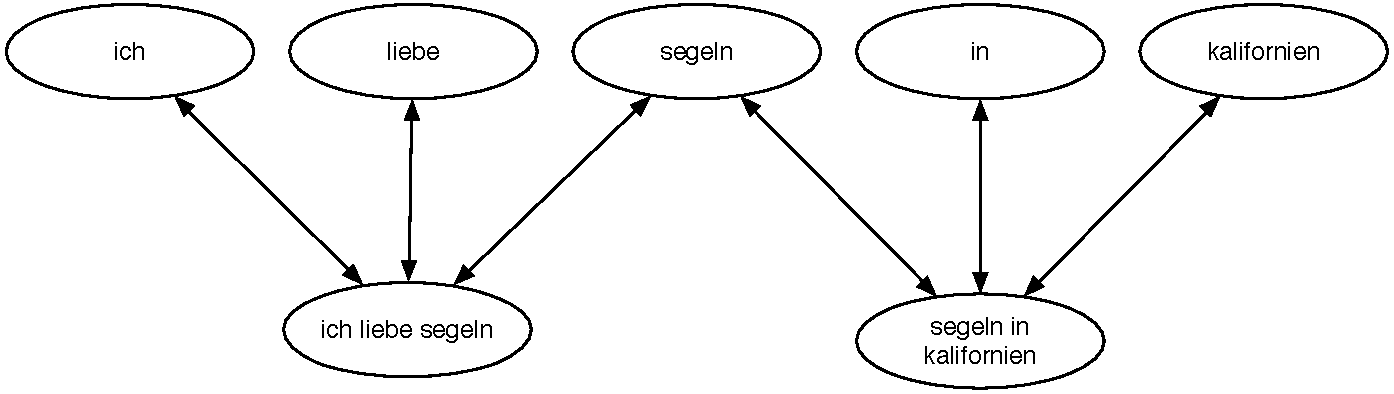
\includegraphics[width=\textwidth]{decomposition}
\caption{Beispielhafter Graphausschnitt nach der Zerlegung}
\label{fig:decomposition}
\end{figure}

Werden diese Begriffe in ihre Einzelwörter zerlegt, entstehen einerseits unter Umständen neue Begriffe, andererseits können in diesem Schritt Zusammenhänge vom Typ \emph{Zerlegung} beziehungsweise \emph{Zusammensetzung} eingefügt werden. Somit sind nach dem Schritt der Zerlegung weitere Informationen über den Kontext, in dem Wörter verwendet werden, verfügbar. \cref{fig:decomposition} zeigt beispielhaft das Ergebnis einer solchen Zerlegung.

\subsection{Ergebnisse}

Durch die Anwendung des Zerlegungsschrittes auf die vorhandenen Begriffe wurden insgesamt \num{38349} neue Knoten und \num{1238900} neue Kanten erzeugt, die für spätere Analyseschritte genutzt werden können.

Die Verteilung der erzeugten Kanten über alle Knoten, die von der Zerlegung betroffen sind, ist in \cref{fig:hist_only_decomposition} als Histogramm dargestellt. Statistische Kennzahlen dieser Verteilung sind in \cref{tab:only_decomposition} aufgeführt.

\begin{figure}[h]
\centering
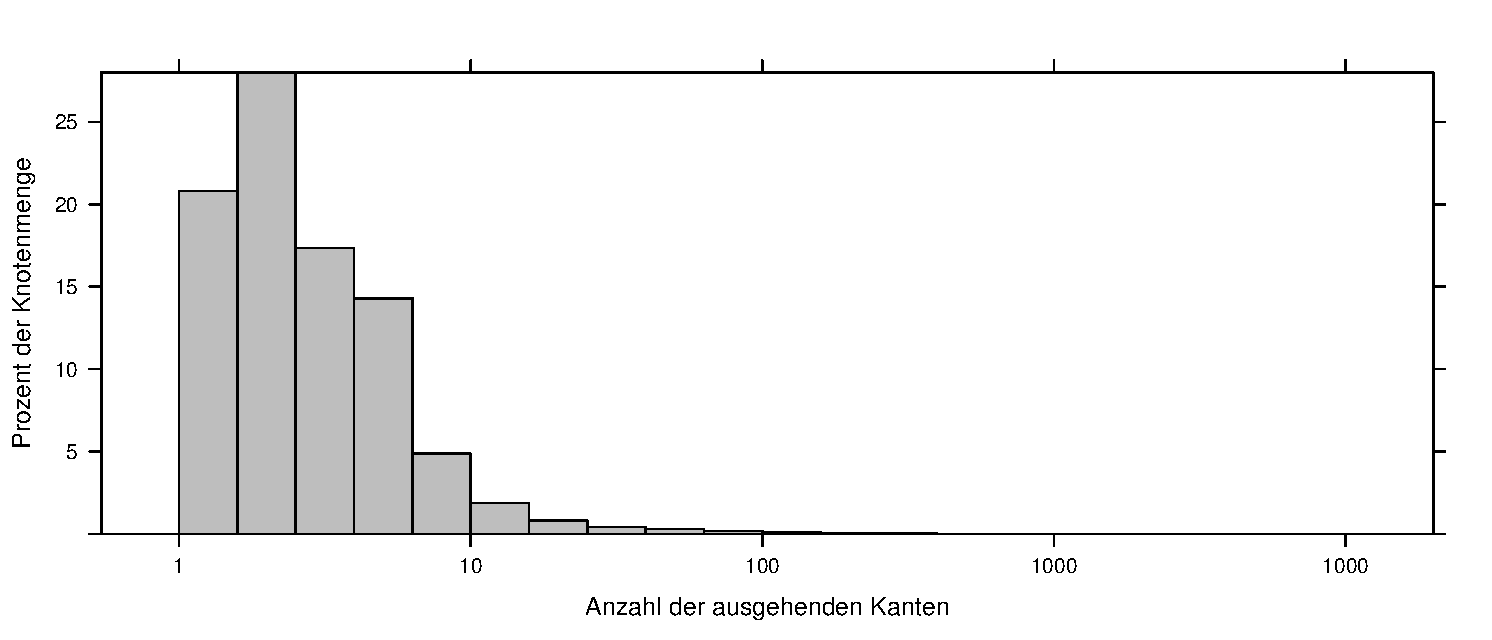
\includegraphics[width=\textwidth]{hist_only_decomposition}
\caption{Histogramm der Verteilung der Zerlegungs-- und Zusammensetzungskanten}
\label{fig:hist_only_decomposition}
\end{figure}

\begin{table}[h]
\centering
\begin{tabular}{lr}
    \toprule
    Kennzahl & Wert \\
    \midrule
    \(min\) & \num{1} \\
    \(Q_{0.25}\) & \num{2} \\
    \(Q_{0.5}\) & \num{2} \\
    \(Q_{0.75}\) & \num{3} \\
    \(max\) &  \num{5215} \\
    \(avg\) &  \num{4,358} \\
    \bottomrule
\end{tabular}
\caption{Statistische Kennzahlen für die Verteilung der Zerlegungs-- und Zusammensetzungskanten}
\label{tab:only_decomposition}
\end{table}

Bei der Zerlegung wurden somit deutlich weniger Kanten pro Knoten erzeugt, als noch bei den Tagging-- und Clicktracking--Daten. Nur ein Viertel der betreffenden Knoten besitzen mehr als drei Kanten vom Typ \emph{Zerlegung} oder \emph{Zusammensetzung}. Der Einfluss der Zerlegung auf den gesamten Datenbestand wird in \cref{lda_results} dargestellt.

Nachdem im Zerlegungsschritt Einzelwörter erzeugt wurden, können diese im folgenden Abschnitt für den Import der Wortschatz--Daten genutzt werden.

\section{Anreicherung mit Wortschatz-Daten}
\label{wortschatz}

Wie in \cref{used_sources} bereits einführend beschrieben, betreibt ein Wortschatz--Projekt \cite{ws2013}. Im Rahmen dieses Projektes wird durch die Analyse von großen Textmengen eine Datenbank deutscher Wörter, deren Bedeutungen, grammatikalische Eigenschaften, Häufigkeiten und Kookkurrenzen in Texten und Beziehungen zu anderen Wörtern aufgebaut. Somit stellt dieses Projekt eine sehr gute Möglichkeit dar, weitere Beziehungen zwischen den schon im Graph vorhandenen Knoten herzustellen. Neben den Daten, die im Spreadshirt--Kontext entstehen, können somit auch allgemeine lexikalische Daten hinzugefügt und für spätere Analysen genutzt werden.

Neben dem Webportal stellt dieses Projekt eine API bereit, über die die Daten des Wortschatzes programmatisch abgefragt werden können. Diese API wurde mittels einer Bibliothek für die Programmiersprache Ruby \cite{wlapi2013} im Rahmen dieser Arbeit für einen weiteren Integrationsschritt zur Link Discovery genutzt. Dazu wurden die Informationen \emph{Grundform}, \emph{Wortformen}, \emph{Kategorien}, \emph{Synonyme} und \emph{Thesaurus--Beziehungen} ausgewertet.

Wie bereits für die anderen Datenquellen, werden im Folgenden auch für den Wortschatz die Schritte des Imports, der Bereinigung, der Reduktion, der Transformation und der Integration beschrieben.

\subsection{Import}

Da für die Anfrage an die Wortschatz--API nur Einzelwörter und keine Wortgruppen genutzt werden können, muss eine Auswahl der anzufragenden Daten getroffen werden. Im Rahmen dieser Arbeit wurden alle Einzelwörter, die zum Zeitpunkt des Importes der Wortschatz--API zur Verfügung standen, ausgewählt. Dabei handelt es sich um \num{197614} einzelne Wörter. Da die Daten in der Datenbank zu diesem Zeitpunkt keine Groß- und Kleinschreibung enthielten, die Wortschatz--API diese jedoch berücksichtigt, wurde jedes Wort jeweils groß und klein geschrieben angefragt. Somit wurde die doppelte Menge an Datensätzen, \num{395228} Dokumente, erzeugt.

Die Ergebnisse wurden mittels eines Ruby--Skriptes in MongoDB importiert. Dabei wurde je angefragtem Wort ein Dokument erzeugt, dass die Informationen des Wortschatzes über dieses Wort enthält. Eines dieser Dokumente ist zu Illustrationszwecken in \cref{lst:wortschatz_import} dargestellt. Das Feld \emph{baseform} enthält die Grundform des Wortes mit der Wortart und \emph{domain} die Kategorien des Wortes.

\begin{lstlisting}[language=json, label={lst:wortschatz_import}, caption={Wortschatz--Dokument nach dem Import}]
{
    "_id" : ObjectId("51f7aa06eba16044e900015a"),
    "string" : "Kopf",
    "baseform" : [ 
        "Kopf", 
        "N"
    ],
    "domain" : [ 
        "Medizin", 
        "Anatomie", 
        "Literarische/Motive/Stoffe/Gestalten", 
        "Körperteile"
    ],
    "synonyms" : [  
        "Chef", 
        "Figur", 
        "Gestalt", 
        "Haupt", 
        "Jemand", 
        "Individuum", 
        "Figur"
    ],
    "thesaurus" : [ 
        "Titel", 
        "Hand", 
        "Kopf", 
        "Mensch", 
        "Gesicht", 
        "Spitze", 
        "Arm", 
        "Gestalt"
    ],
    "wordforms" : [ 
        "Kopf", 
        "Köpfe", 
        "Köpfen", 
        "Kopfes", 
        "Kopfs"
    ]
}
\end{lstlisting}

Hierbei ist zu beachten, dass nicht alle Attribute bei allen Wörtern vorhanden sind. Dies hängt davon ab, ob der Wortschatz die Informationen zur Verfügung stellen kann. Somit ist es auch möglich, dass Dokumente erzeugt werden, die keine zusätzlichen Informationen enthalten.

\subsection{Bereinigung}

Zur Bereinigung der importierten Wortschatz--Daten muss in einem ersten Schritt die Groß- und Kleinschreibung entfernt werden, da diese an erster Stelle nur für die Anfragen an die API wieder in den Datenbestand eingeführt wurde.

Weiterhin werden die Kategorien ``Vorname'' und ``Nachname'' entfernt, da diese an über \num{25000} Wörter vergeben sind und somit für die Verwendung zur Link Discovery ungeeignet sind und zu viele irrelevante Kanten erzeugen würden.

Ein letzter Bereinigungsschritt besteht in der Veränderung des Formates der Grundform des Wortes. Die Wortschatz--API liefert lediglich ein Array, in dem das erste Element die Grundform und das zweite Element die Wortart ist. Zur Bereinigung wird diese Eigenschaft in ein geeignetes JSON--Format überführt, welches in \cref{lst:word_baseform} dargestellt ist.

\begin{lstlisting}[language=json, label={lst:word_baseform}, caption={Grundform eines Wortes}]
{
    _id: ...,
    string: "Kopfs",
    baseform: {
        word: "Kopf",
        type: "N"
    }
}
\end{lstlisting}

\subsection{Reduktion}

Der Reduktionsschritt besteht in der Zusammenführung von Dokumenten mit gleichen Wörtern, welche im Bereinigungsschritt entstanden sind. Wie schon bei der Reduktion der Tagging--Daten, muss auch hierbei das Entstehen neuer Duplikate vermieden werden. Dies bedeutet, dass die gefundenen Wortbeziehungen ebenfalls zusammengeführt werden, wobei jedes verbundene Wort nur einmal enthalten sein darf. Die Reduktion ist beispielhaft in \cref{fig:wortschatz_reduction} dargestellt. Dabei ist zu beachten, dass bei der Zusammenführung mehrere Grundformen entstehen können, wodurch dieses Attribut in ein Array umgewandelt wird.

\begin{figure}
\centering
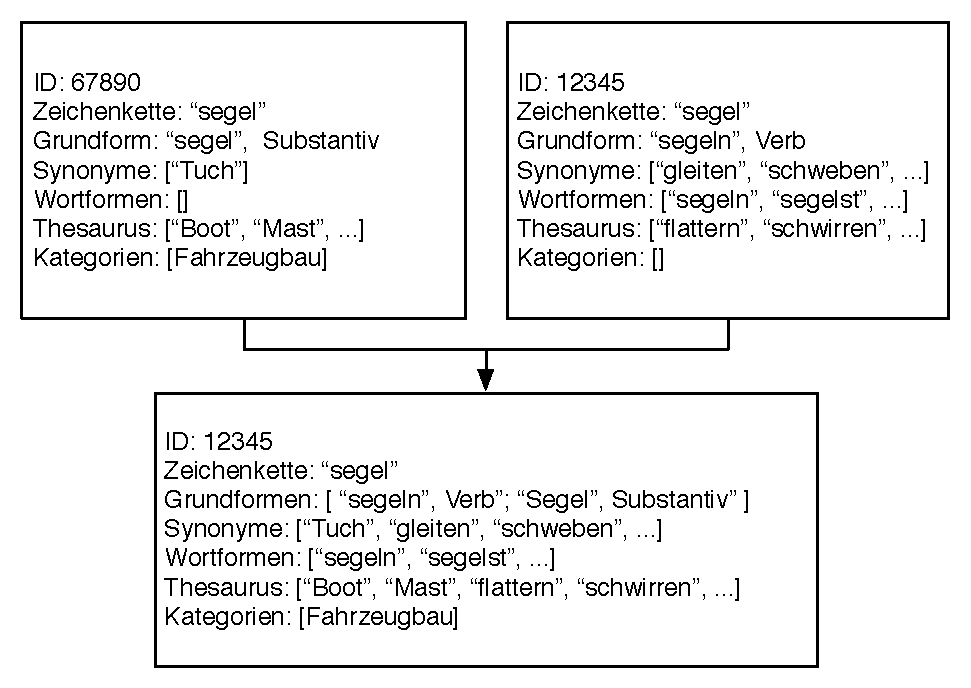
\includegraphics[width=0.8\textwidth]{wortschatz_reduction}
\caption{Reduktion der Wortschatz--Daten}
\label{fig:wortschatz_reduction}
\end{figure}

Durch die Reduktion wird die Anzahl der Dokumente auf die Hälfte reduziert und beträgt danach \num{197614}.

\subsection{Transformation}

Die Transformation der Wortschatz--Daten besteht, wie bereits bei den anderen Datenquellen, in einer Überführung in eine Graph--Datenstruktur. 

Die Knoten sind alle Wörter, die durch die Benutzung der Wortschatz--API bekannt sind. Dazu zählen einerseits sowohl die angefragten Wörter, als auch die verbundenen Wörter, die die API liefert.

Die Kanten werden jeweils für die Attribute \emph{Synonyme}, \emph{Thesaurus}, \emph{Grundform} und \emph{Wortformen} erzeugt und besitzen die entsprechenden Kantentypen. Sie enthalten keine weiteren Attribute, da über diese Beziehungen keine weiteren Informationen verfügbar sind.
\begin{figure}
\centering
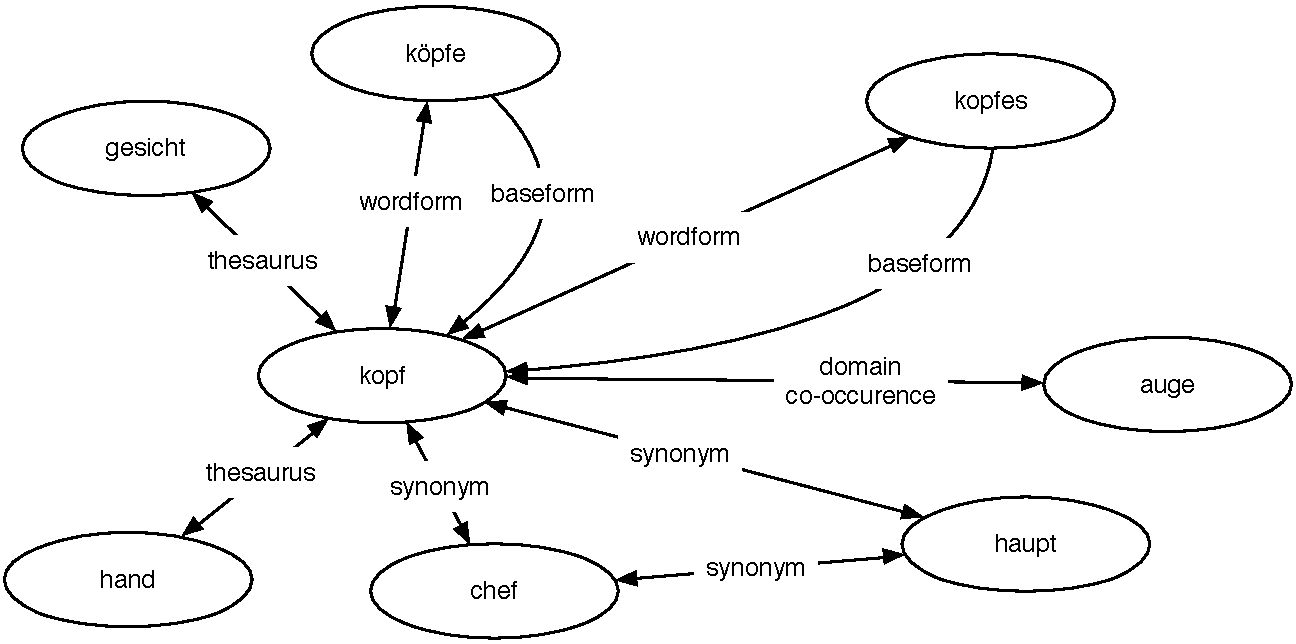
\includegraphics[width=\textwidth]{wortschatz_transformation}
\caption{Wortschatz--Daten in Graphenform}
\label{fig:wortschatz_transformation}
\end{figure}

Einen Sonderfall stellen die Kategorien der Wörter dar. Diese können in der vorliegenden Form nicht zur Link Discovery genutzt werden. Daher werden diese Daten mittels der Ermittlung von Kookkurrenzen umgeformt. Von Interesse ist, wie oft Paare von Wörtern 
in gemeinsame Kategorien eingeordnet sind. 

Somit werden bei der Transformation mittels MapReduce (siehe \cref{mapreduce_cooccurence}) Kanten mit den Kookkurrenzmaßen Dice, Jaccard und Kosinus erzeugt.

Zusammenfassend werden bei der Transformation demnach Kanten mit den Typen \emph{Synonym}, \emph{Thesaurus}, \emph{Wortform}, \emph{Grundform} und \emph{Kategorie--Kookkurrenz} erzeugt. In \cref{fig:wortschatz_transformation} wird beispielhaft ein Ausschnitt des resultierenden Graphen gezeigt. Dabei fällt auf, dass mit Ausnahme der Grundform--Kanten jede Kante in beide Richtungen existiert. Dies ist der Art der Beziehungen geschuldet, da diese in beide Richtungen gültig sind.

\subsection{Integration}

Zur Integration wird der im Transformationsschritt erzeugte Graph mit dem Zielgraphen vereinigt. Diese Vereinigung wird analog zur Integration der Clicktracking--Daten in \cref{click_integration} durchgeführt.

Insgesamt wurden dadurch \num{145023} neue Knoten und \num{50227965} neue Kanten erzeugt.  Dabei entfallen \num{48399466} Kanten auf Kookkurrenz von Kategorien, \num{550270} Kanten auf Wortformen, \num{149381} Kanten auf Grundformen, \num{279118} Kanten auf Synonyme und \num{849730} Kanten auf Thesaurus--Beziehungen.

Nachdem alle vorgenommen Schritte zur Link Discovery beschrieben wurden, beschäftigt sich der nächste Abschnitt mit einer Zusammenfassung der Ergebnisse.

\subsection{Ergebnisse}

\section{Prioisierung der Beziehungen}

Im folgenden Kapitel werden die vorgenommenen Optimierungsmaßnahmen und die damit einhergehende Evaluierung der Ergebnisse der Link Discovery beschrieben. Dazu gehören der gewählte Ansatz zur Optimierung, eine Erläuterung evolutionärer Algorithmen und deren Einsatz zur Optimierung sowie die Darstellung und Auswertung der Ergebnisse.

Zuerst muss definiert werden, welcher Aspekt genau optimiert werden soll. Die in \cref{link_discovery} beschriebenen Schritte haben einen Graphen erzeugt, in dem neun verschiedene Kantentypen existieren. Diese lauten \emph{Tag--Kookkurrenz}, \emph{Klick--Kookkurrenz}, \emph{Zusammensetzung}, \emph{Wortform}, \emph{Grundform}, \emph{Synonym}, \emph{Thesaurus--Beziehung}, \emph{Kategorie--Kookkurrenz} und \emph{Zerlegung}.

Werden nun inhaltlich relevante Nachbarn zu einem gegebenen Begriff gesucht, müssen alle ausgehenden Kanten des entsprechenden Knotens nach Relevanz geordnet werden. Dazu muss jede Kante ein Kantengewicht besitzen. Die Addition aller Kantengewichte zwischen zwei Knoten stellt somit das Maß für ihre Nähe dar.

Die Kanten vom Typ Kookkurrenz besitzen bereits aufgrund der angegebenen Kookkurrenzmaße Kantengewichte. Jedoch muss hierbei festgelegt werden, welches Maß für das Kantengewicht herangezogen werden und in welchem Verhältnis zu den Gewichten anderer Kantentypen es stehen soll.

Somit hängt die Berechnung der Relevanz zwischen zwei Knoten von zwölf Parametern ab. Jedem Kantentyp muss ein Gewicht zugewiesen und außerdem muss eine Auswahl von drei Kookkurrenzmaßen getroffen werden. Die Optimierung und Evaluierung dieser berechneten Relevanz ist Gegenstand dieses Kapitels.

Die Einschätzung, ob die Ordnung der Nachbarn eine Ordnung der Relevanz zum Ausgangsbegriff darstellt, kann nicht automatisch, sondern nur von Menschen, getroffen werden. Somit stellt die Bewertung einer bestimmten Gewichtung der Kanten auch eine Evaluierung der Kantentypen dar.
Generell kann außerdem nicht davon ausgegangen werden, dass eine einmal gefundene Gewichtung der Kanten für alle Knoten des Graphen verwertbare Ergebnisse erzeugt. Daher sollte die Optimierung nicht global, sondern für jeden Knoten einzeln erfolgen. Aufgrund der hohen Knotenanzahl wurde sich hierzu auf eine stichprobenartige Auswahl der Knotenmenge beschränkt.

Durch die Notwendigkeit menschlicher Beteiligung und der großen Anzahl an Parametern ist eine Optimierung mittels des Ausprobierens aller Fälle nicht möglich. Außerdem kann die Einschätzung, welche Kantengewichtungen relevante Ergebnisse erzeugen, stark von Mensch zu Mensch variieren. Stattdessen muss zur Optimierung ein Ansatz gefunden werden, der sich einer, für den Großteil der Personen, optimalen Gewichtung möglichst nähert. 

Im Rahmen dieser Arbeit wurde aus den genannten Gründen ein Optimierungsansatz mittels interaktiver evolutionärer Algorithmen gewählt. Die Grundlagen evolutionärer Algorithmen und die gewählte Implementierung werden in den folgenden Abschnitten beschrieben.

\subsection{Vorgehensweise}
\label{evo_implementation}

Nachdem im vorhergehenden Abschnitt die Grundlagen und Komponenten evolutionärer Algorithmen beschrieben wurden, werden im Folgenden die für die Optimierung der Link Discovery--Ergebnisse angewendeten Methoden erläutert.

Zunächst soll die Methode zur Auswahl der Stichproben erläutert werden. Insgesamt wurden fünfzehn Knoten ausgewählt, deren Beziehungen optimiert werden sollen. Die Auswahl der Knoten richtete sich nach der Popularität von Suchbegriffen auf der Website von Spreadshirt. Dazu wurden alle Begriffe mit mehr als eintausend Suchen herangezogen und diese nach Häufigkeit der Suchen geordnet. Daraus wurden zufällig je fünf Begriffe bis zum unteren Quartil, fünf Begriffe zwischen unterem und oberen Quartil und fünf Begriffe über dem oberen Quartil ausgewählt. Die ausgewählten Begriffe, deren Kantengewichtungen lokal optimiert werden sollen, lauten: \emph{Kopfkissenbezug}, \emph{Student}, \emph{Volkswagen}, \emph{Marathon}, \emph{Wow}, \emph{Krankenschwester}, \emph{Mountainbike}, \emph{Hammer}, \emph{Polska}, \emph{Regenbogen}, \emph{Minecraft}, \emph{Kind}, \emph{Dubstep}, \emph{Leipzig} und \emph{Valentinstag}.

Ziel dieser Auswahl war, eine möglichst vielfältige Verteilung der einzelnen Kantentypen zu erreichen, aus welcher sich nach Durchführung der Optimierung möglicherweise Erkenntnisse ableiten lassen, ob die Optimierung nur lokal oder auch global durchgeführt werden kann.

Nach Auswahl der Stichproben muss der Genotyp der am evolutionären Algorithmus teilnehmenden Individuen spezifiziert werden. Daraufhin muss definiert werden, wie die Komponenten des Algorithmus zu implementieren sind.

\subsection{Genotyp}

Jeder Lösungskandidat wird durch die Werte der zwölf Parameter definiert, die die Gewichtung der Kantentypen untereinander beeinflussen. Daher wird jedes Individuum als Objekt repräsentiert, dass zwölf Attribute besitzt. Davon sind neun Attribute reellwertig und drei Attribute vom Aufzählungstyp \emph{Kookkurrenzmaß}.

\begin{figure}
\centering
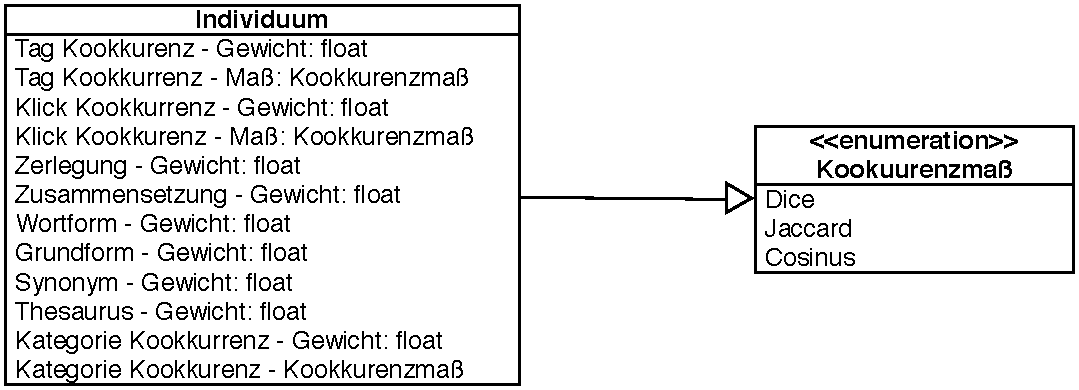
\includegraphics[width=0.9\textwidth]{genotype}
\caption{UML--Klassendiagramm des gewählten Genotyps}
\label{fig:genotype}
\end{figure}

Die reellwertigen Attribute stellen ein Gewicht des jeweiligen Kantentyps dar. Sie können nur relativ zu den anderen Kantengewichten betrachtet werden und somit nur im Rahmen der Optimierung von Interesse. Der Wertebereich dieser Attribute wird auf das Intervall \((0,1)\) eingeschränkt. Die Kookkurrenzmaße entsprechen den in \cref{measures} genannten, also \emph{Dice}, \emph{Jaccard} und \emph{Kosinus}. Der Genotyp ist in \cref{fig:genotype} als UML--Klassendiagramm und in \cref{lst:genotyope} beispielhaft in JSON--Notation dargestellt.

\begin{lstlisting}[language=json, label={lst:genotyope}, caption={Beispiel für ein Individuum}]
{
    "tagCoOccMeasure" : 0,
    "tagCoOccWeight" : 0.6878115427680314,
    "clickCoOccMeasure" : 2,
    "clickCoOccWeight" : 0.1533144270069897,
    "synonymWeight" : 0.2355003503616899,
    "thesaurusWeight" : 0.9918724503368139,
    "baseformWeight" : 0.2843543488997966,
    "wordformWeight" : 0.93317318148911,
    "sharedDomainsMeasure" : 2,
    "sharedDomainsWeight" : 0.462230023695156,
    "compositionWeight" : 0.07963851140812039,
    "decompositionWeight" : 0.4740817183628678
}
\end{lstlisting}

\subsection{Initialisierung}

Im Initialisierungsschritt wird die anfängliche Population für jede der Stichproben gebildet. Dazu muss zuerst eine geeignet erscheinende Populationsgröße festgelegt werden.

In jeder Generation müssen im Evaluierungsschritt alle Individuen bewertet werden. Wie einführend bereits erläutert wurde, kann dies nur mit menschlicher Interaktion erfolgen. Somit sollte die Populationsgröße möglichst gering sein, um mit der gleichen Anzahl Bewertungen eine größere Anzahl von Generationen zu durchlaufen. Dies geschieht auf Kosten der Diversität in der Population. Jedoch wurde im Rahmen dieser Arbeit dieser Ansatz gewählt, um möglichst viele Möglichkeiten zu haben, die Parameter zu optimieren.

Es wurde eine Populationsgröße von zehn Individuen je Stichprobe gewählt. Somit müssen in jeder Generation einhundertfünfzig Individuen bewertet werden. Bei der Initialisierung wurden die Variablen jedes erzeugten Individuums zufällig gewählt.

\subsection{Selektion}

Die Bestimmung einer Fitnessfunktion für die Optimierung der Link Discovery gestaltet sich durch die Notwendigkeit menschlicher Beurteilung als schwierig. Eine solche Fitnessbestimmung müsste derart erfolgen, dass ein Benutzer jedem Individuum einen reellwertigen Fitnesswert zuweist. Dies gestaltet ist jedoch auf Grund der hohen Anzahl von Individuen nicht praktikabel.

Die umgesetzte Selektion erfolgt durch die Durchführung von Wettkämpfen. Hierzu werden in jeder Generation je fünf Paare von Individuen gebildet. Diese Paarungen stellen die Wettkämpfe dar, bei denen der Benutzer den Gewinner bestimmt. Alle Gewinner werden selektiert und im Reproduktionsschritt weiter verwendet.

Der Vorteil dieses Vorgehens ist, dass der Benutzer nur jeweils zwei Lösungskandidaten vergleichen muss, anstatt direkt fünf der zehn Individuen auszuwählen. Somit verringert sich der zu einem Zeitpunkt zu leistende kognitive Aufwand für die Selektion.

\begin{figure}
\centering
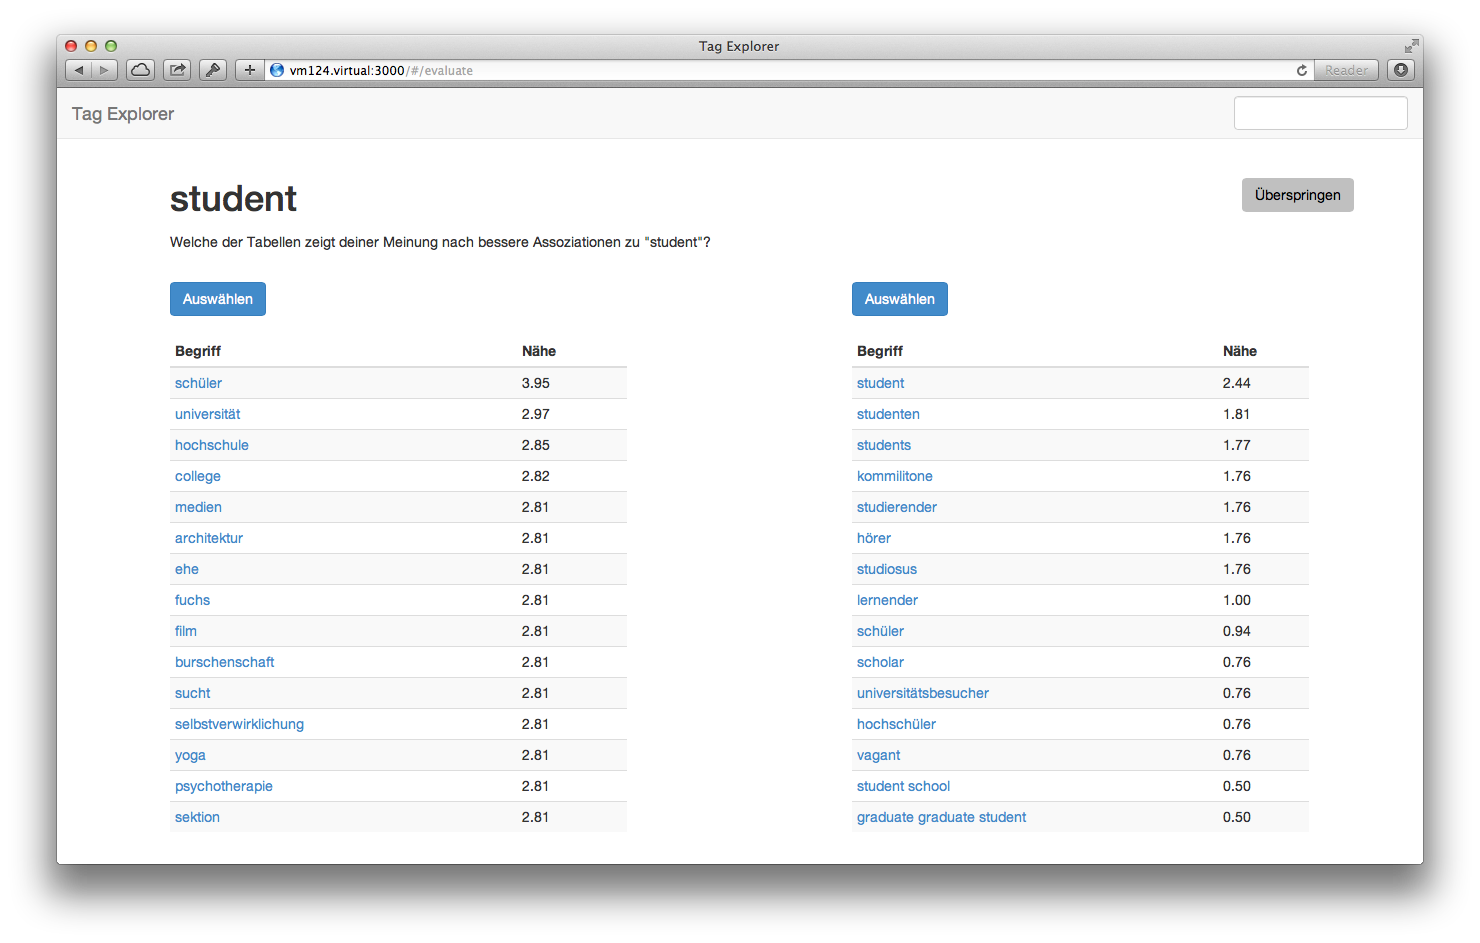
\includegraphics[width=\textwidth]{eva_interface}
\caption{Oberfläche zur interaktiven Selektion}
\label{fig:eva_interface}
\end{figure}

Zur Selektion besucht der Benutzer eine Website, auf der ihm zwei Lösungskandidaten für eine Stichprobe präsentiert werden. Die Lösungskandidaten werden in Form von Listen von je fünfzehn Begriffen dargestellt, die die mit der jeweiligen Kantengewichtung erzeugten nächsten Nachbarn des Begriffes sind. Diese Oberfläche ist in \cref{fig:eva_interface} als Screenshot abgebildet. Nach Auswahl eines Gewinners wird dem Nutzer der nächste Wettkampf präsentiert.

Am Selektionsprozess kann sich jeder interessierte Benutzer beteiligen. Dieses Vorgehen wurde gewählt, um ein möglichst breites Spektrum an Meinungen bezüglich der Güte der Verbindungen zu erhalten.

Durch die direkte Auswahl beträgt die Reproduktionswahrscheinlichkeit für die ausgewählten Individuen eins und für die nicht ausgewählten Individuen Null \cite{sd2012}. Die gewählten Reproduktionsverfahren werden im nächsten Abschnitt beschrieben.

\subsection{Reproduktion}

Die fünf selektierten Individuen werden zur Reproduktion herangezogen, um fünf neue Individuen zu erzeugen, damit die Populationsgröße für die nächste Selektion wieder auf zehn Individuen steigt. Dazu werden die selektierten Individuen zuerst rekombiniert, um fünf Kindindividuen zu erzeugen, welche dann durch Mutation verändert werden.

\paragraph{Rekombination}

Als Verfahren zur Rekombination wurde der \emph{Ein--Punkt--Crossover} \cite{kw2007} gewählt. Dazu werden zufällig zwei Elternindividuen ausgewählt und ein zufälliger Crossover--Punkt berechnet. Werden die Genotypen der beiden Elternindividuen als Arrays dargestellt, werden bis zum Crossover--Punkt die Variablen des ersten Individuums, nach dem Crossover--Punkt die Variablen des zweiten Individuums übernommen. Der Crossover ist in \cref{fig:crossover} dargestellt.

\begin{figure}
\centering
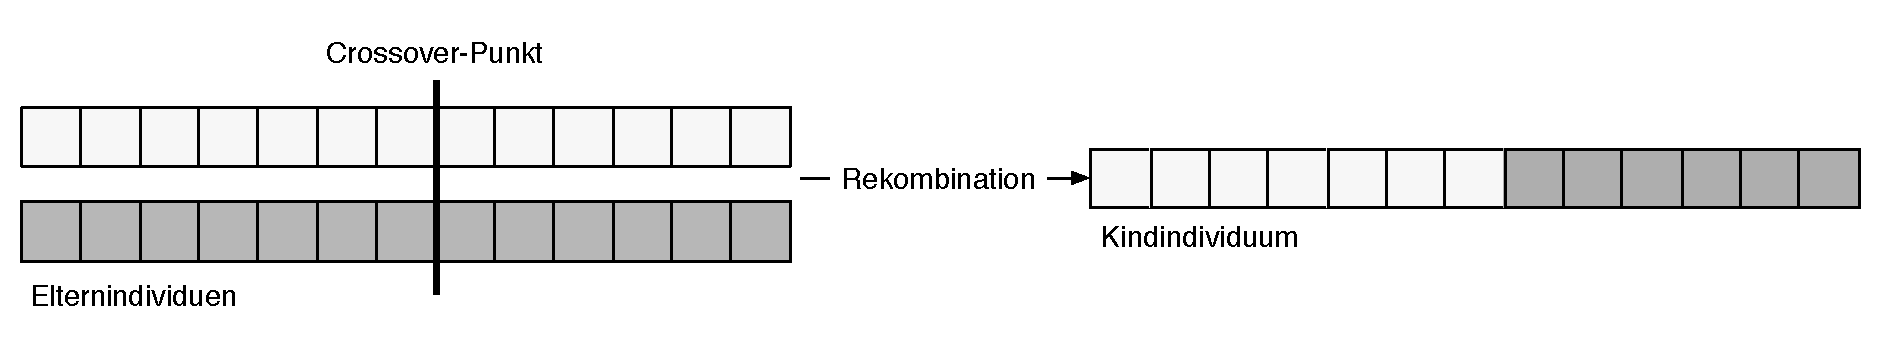
\includegraphics[width=\textwidth]{crossover}
\caption{Ein--Punkt--Crossover}
\label{fig:crossover}
\end{figure}

\paragraph{Mutation}

Zur Mutation der reellwertigen Kantengewichtungen wurde das Verfahren der \emph{Gauß-Mutation} \cite{kw2007} gewählt. Dabei wird zu jeder reellwertigen Variablen des Genotyps ein normalverteilter Zufallswert addiert. Verlässt der entstehende Wert das zulässige Intervall, so wird er auf die entsprechende Intervallschranke angepasst. Die Gauß-Mutation macht daher große Änderungen der Variable möglich, aber weniger Wahrscheinlich als kleine Änderungen. Sie eignet sich somit gut, um Diversität in der Population zu erzeugen. Konkret wurde in der Umsetzung der Optimierung eine auf das Intervall \((0,1)\) angepasste Normalverteilung mit Erwartungswert \(\mu=0\) und Varianz \(\sigma=0.5\) gewählt. Die Variablen für die Kookkurrenzmaße werden nicht mutiert.

Nachdem in diesem Abschnitt die konkrete Umsetzung der Optimierung mittels interaktiver evolutionärer Algorithmen beschrieben wurde, folgt im nächsten Abschnitt die Darstellung und Diskussion der Ergebnisse.

\subsection{Ergebnisse}

Die Optimierung wurde über insgesamt \num{13} Generationen durchgeführt. Somit wurden über alle Stichproben hinweg \num{975} Selektionen von Benutzern vorgenommen. Die Benutzer waren allesamt Mitarbeiter von Spreadshirt. Aufgrund der anonymen Teilnahme lässt sich nicht angeben, wie viele Einzelpersonen an der Optimierung teilgenommen haben.

\subsection{Kantengewichte}

Da nach jeder Selektion je Stichprobe fünf Individuen in der Population verbleiben, werden zunächst deren Kantengewichtungen untersucht. \cref{tab:winners_total} zeigt für jede Variable aus dem Genotyp den Median der in der dreizehnten Generation selektierten Individuen. Das Kantengewicht für den Typ \emph{Zerlegung} ist nicht in der Tabelle enthalten, da es sich bei den Stichproben nur um Einzelwörter handelt.

\begin{table}
\centering
\begin{tabular}{lcccccccc}
    \toprule
    Stichprobe & \(k_t\) & \(k_{kl}\) & \(s\) & \(t\) & \(g\) & \(w\) & \(k_{ka}\) & \(zu\) \\
    \midrule
    Dubstep & 0.85 & 0.60 & 0.53 & 0.77 & 1.00 & 1.00 & 1.00 & 0.48 \\
    Hammer & 0.81 & 0.56 & 0.88 & 0.45 & 1.00 & 0.89 & 0.00 & 0.59 \\
    Kind & 0.58 & 0.22 & 0.84 & 1.00 & 0.66 & 0.00 & 0.01 & 0.00 \\
    Kopfkissenbezug & 0.34 & 0.00 & 0.00 & 0.60 & 0.77 & 0.93 & 0.26 & 0.93 \\
    Krankenschwester & 1.00 & 0.20 & 0.28 & 0.60 & 0.70 & 0.88 & 0.59 & 0.33 \\
    Leipzig & 0.69 & 1.00 & 0.66 & 0.01 & 0.41 & 0.00 & 0.17 & 1.00 \\
    Marathon & 0.62 & 0.70 & 0.23 & 0.41 & 0.69 & 1.00 & 0.00 & 0.95 \\
    Minecraft & 0.71 & 0.34 & 0.31 & 0.38 & 0.74 & 1.00 & 0.00 & 1.00 \\
    Mountainbike & 0.34 & 0.48 & 0.00 & 0.00 & 1.00 & 1.00 & 0.85 & 0.00 \\
    Polska & 0.63 & 0.25 & 0.86 & 0.97 & 0.24 & 1.00 & 0.00 & 0.00 \\
    Regenbogen & 1.00 & 0.43 & 0.36 & 0.47 & 0.00 & 0.26 & 0.61 & 0.52 \\
    Student & 0.67 & 0.15 & 0.38 & 0.84 & 0.78 & 0.70 & 0.72 & 0.33 \\
    Valentinstag & 1.00 & 0.44 & 0.80 & 0.24 & 0.53 & 0.58 & 0.70 & 1.00 \\
    Volkswagen & 0.47 & 1.00 & 0.11 & 0.51 & 1.00 & 0.89 & 0.14 & 0.30 \\
    Wow & 0.08 & 1.00 & 0.93 & 0.21 & 1.00 & 0.54 & 0.53 & 0.68 \\
    \bottomrule
\end{tabular}
\caption{Mediane der Kantengewichte nach der finalen Selektion}
\caption*{
    \begin{tabular}{ll}
        \(k_t\) & Tag--Kookkurrenz\\
        \(k_{kl}\) & Klick--Kookkurrenz\\
        \(s\) & Synonyme \\
        \(t\) & Thesaurus \\
        \(g\) & Grundform \\
        \(w\) & Wortform \\
        \(k_{ka}\) & Kategorie--Kookkurrenz\\
        \(zu\) & Zusammensetzung\\
    \end{tabular}
}
\label{tab:winners_total}
\end{table}

Bei Betrachtung dieser Ergebnisse fällt auf, dass sich die Gewichtungen der Kanten von Stichprobe zu Stichprobe stark unterscheiden. Somit bestätigt sich die Vermutung, dass eine globale Optimierung der Kantengewichtungen keine sinnvollen Ergebnisse erzielt. Jedoch ergaben sich für die Typen \emph{Wortform} und \emph{Grundform} in allen Stichproben relativ hohe Gewichte.



\subsection{Kookkurrenzmaße}

In \cref{tab:measures_each} sind für alle Stichproben die nach der letzten Selektion jeweils am häufigsten in der Population auftretenden Kookkurrenzmaße aufgeführt.

\begin{table}
\centering
\begin{tabular}{llll}
    \toprule
    Stichprobe & Tags & Klicks & Kategorien \\
    \midrule
    Dubstep & Jaccard & Dice & Dice \\
    Hammer & Dice & Dice & Kosinus \\
    Kind & Kosinus & Dice & Kosinus \\
    Kopfkissenbezug & Dice & Dice & Kosinus \\
    Krankenschwester & Jaccard & Dice & Dice \\
    Leipzig & Jaccard & Jaccard & Kosinus \\
    Marathon & Dice & Dice & Jaccard \\
    Minecraft & Dice & Dice & Kosinus \\
    Mountainbike & Kosinus & Jaccard & Jaccard \\
    Polska & Jaccard & Dice & Kosinus \\
    Regenbogen & Dice & Dice & Jaccard \\
    Student & Dice & Dice & Dice \\
    Valentinstag & Dice & Jaccard & Kosinus \\
    Volkswagen & Kosinus & Dice & Dice \\
    Wow & Jaccard & Dice & Dice \\
    \bottomrule
\end{tabular}
\caption{Häufigste Kookkurrenzmaße nach der finalen Selektion}
\label{tab:measures_each}
\end{table}

\section{Auswertung der Ergebnisse}
\label{lda_results}

Im folgenden Abschnitt werden die quantitativen Ergebnisse der Link Discovery zusammenfassend dargestellt und diskutiert.

\begin{table}
\centering
\begin{tabular}{lrcr}
    \toprule
    Schritt & Knoten & \phantom{abc} & Kanten \\
    \midrule
    Tags & \num{314351} && \num{21834868} \\
    Clicktracking & \num{78237} && \num{310860} \\
    Zerlegung & \num{38349} && \num{1238900} \\
    Wortschatz & \num{145023} && \num{50227965} \\
    \midrule
    Gesamt & \num{575960} && \num{73612593} \\
    \bottomrule
\end{tabular}
\caption{Quantitative Ergebnisse der Link--Discovery--Schritte}
\label{tab:discovery_amounts}
\end{table}

\cref{tab:discovery_amounts} führt für jeden Schritt die hinzugefügten Knoten und Kanten sowie die nach Durchführung der Link Discovery insgesamt im Graphen enthaltene Datenmenge auf. Dabei zeigt sich, dass die Integration der Daten des Wortschatzes mit Abstand die meisten neuen Kanten in den Graphen eingefügt hat. 

Bei der Verwendung der Clicktracking--Daten wurden im Verhältnis wenig neue Knoten und Kanten erzeugt. Dies ist im Wesentlichen auf den zum Zeitpunkt des Importes noch geringen Datenbestand zurückzuführen. Daher sollte dieser Schritt zukünftig wiederholt werden, da mit der längeren Laufzeit des Clicktracking--Systems auch ein größeres Potential für neue Verknüpfungen vorhanden ist.

Neben der absoluten Anzahl der Knoten und Kanten sind bei einer Betrachtung der quantitativen Ergebnisse auch die Anzahl der Kanten, die von einem Knoten ausgehen, von Interesse. \cref{tab:discovery_edges_per_node} zeigt die Entwicklung der Kantenanzahl pro Knoten nach jedem Link--Discovery--Schritt. Dabei sind Minimum, das untere, mittlere (Median) und obere Quartil, das Maximum und der Durchschnitt dargestellt, um die Verteilung der Kantenanzahl zu verdeutlichen.

\begin{table}
\centering
\begin{tabular}{lrrrrrr}
    \toprule
    Schritt & \(min\) & \(Q_{0.25}\) & \(Q_{0.5}\) & \(Q_{0.75}\) & \(max\) & \(avg\) \\
    \midrule
    Tags & \num{0} & \num{8} & \num{15} & \num{26} & \num{35170} & \num{69,64} \\
    Clicktracking & \num{0} & \num{3} & \num{10} & \num{23} & \num{35170} & \num{56,41} \\
    Zerlegung & \num{0} & \num{4} & \num{11} & \num{24} & \num{37940} & \num{54,26} \\
    Wortschatz & \num{0} & \num{2} & \num{8} & \num{23} & \num{38380} & \num{127,8} \\
    \bottomrule
\end{tabular}
\caption{Entwicklung der Anzahl der Kanten von einem Knoten ausgehend}
\label{tab:discovery_edges_per_node}
\end{table}

Auffällig ist hierbei, dass die Integration von Clicktracking- und Wortschatz--Daten zu einer Herabsetzung des Medians führten. Dies bedeutet, dass nach Durchführung dieser Schritte verhältnismäßig weniger viel verbundene Knoten im Datenbestand existierten als davor. Jedoch deutet die Entwicklung des Durchschnittes nach der Integration der Wortschatz--Daten darauf hin, dass die Knotenanzahl viel verbundener Knoten nach diesem Schritt deutlich größer geworden ist.

Das Absinken des Durchschnittes nach Integration der Clicktracking--Daten kann in der geringen Menge der Daten begründet werden. Durch die geringe Anzahl von Kookkurrenzen konnten viel verbundene Knoten keinen relevanten Zugewinn an Verbindungen verzeichnen, während für wenig verbundene Knoten verhältnismäßig mehr neue Verbindungen hinzukamen.

Generell lässt sich festhalten, dass die Anzahl viel verbundener Knoten gemessen an der Gesamtanzahl relativ klein ist. Die Auswirkungen dessen hängen jedoch stark von der Anwendung der Daten ab und sind im Rahmen dieser Arbeit nicht beurteilbar.

Nach der quantitativen Auswertung der Link--Discovery-–Schritte wird im nächsten Kapitel die Optimierung der Kantengewichtungen und die Evaluierung der erzeugten Kanten beschrieben.

\section{Zusammenfassung}